\documentclass{article}

\usepackage[final]{neurips_2019}

\usepackage[utf8]{inputenc}
\usepackage[T1]{fontenc}
\usepackage{hyperref}
\usepackage{url}
\usepackage{booktabs}
\usepackage{amsfonts}
\usepackage{nicefrac}
\usepackage{microtype}
\usepackage{graphicx}
\usepackage{xcolor}
\usepackage{lipsum}

\newcommand{\note}[1]{\textcolor{blue}{{#1}}}

\title{
  Lost in Legalese: NLP for Privacy Risk Detection \\
  \vspace{1em}
  \small{\normalfont Stanford CS224N Custom Project}  % Select one and delete the other
}

\author{
  Ray Hu \\
  Department of Computer Science \\
  Stanford University \\
  \texttt{rayhu@stanford.edu} \\
  \And
  Benjamin Ward \\
  Institute for Computational and Mathematical Engineering \\
  Stanford University \\
  \texttt{wardb@stanford.edu} \\  
  \And
  Basant Khalil \\
  Department of Computer Science \\
  Stanford University \\
  \texttt{bkhalil@stanford.edu}
}
  % Examples of more authors
%   \And
%   Name \\
%   Department of Computer Science \\
%   Stanford University \\
%   \texttt{name@stanford.edu} \\
%   \And
%   Name \\
%   Department of Computer Science \\
%   Stanford University \\
%   \texttt{name@stanford.edu}


\begin{document}

\maketitle

% \begin{abstract}
%   Required for final report
% \end{abstract}


% \note{This template is built on NeurIPS 2019 template\footnote{\url{https://www.overleaf.com/latex/templates/neurips-2019/tprktwxmqmgk}} and provided for your convenience.}


\section{Project Information}

\begin{itemize}
    % \item External collaborators (if you have any):
    \item $\mathbf{Project}$ $\mathbf{type}$: custom project.
    \item $\mathbf{Mentor}$: Jing Huang (hij@stanford.edu) will be the project mentor.
\end{itemize}


\section{Research paper summary (max 2 pages)}

\begin{table}[h]
    \centering
    \begin{tabular}{ll}
        \toprule
        \textbf{Title} & Know What You Don't Know: User's Rights in Online Terms and Conditions \\
        \midrule
        \textbf{Venue} & Stanford CS-224N Winter 2025 \\
        \textbf{Year}  & 2025 \\
        \textbf{URL}   & \url{https://github.com/AI-knows-your-rights/t-c-ranker} \\
        \bottomrule
    \end{tabular}
    \vspace{1em}
    \caption{Presentation of Related Research Paper
    }
    % ~\cite{rajpurkar2018know}.
\end{table}

\paragraph{Background.}
Legal language is one of the most complex and sophisticated forms of natural language. A tragic 2024 case brought this issue to public attention: a woman passed away at Disney Park, and the company argued that her family had waived their right to sue because she had accepted the terms and conditions (T\&C) when she signed up for a trial of Disney+ stream back in 2019. The legal clause, buried in fine print, favored the company, highlighting how consumers often unknowingly forfeit their rights.

\paragraph{Summary of contributions.}
Our project aims to develop an NLP model that can summarize and rate T\&C, making them easier for consumers to understand. We have identified a community-annotated dataset containing 500 companies' T\&C. It includes manual analyses of qualified attorney volunteers, providing a strong foundation for classification and summarization. The dataset has been used to make a browser extension. Here is the screenshot. Google T\&C is ranked as grade E as it includes many clauses that don’t respect users' privacy. On the contrary, DuckDuckGo has an excellent rating. However, the manual analysis is expensive, slow, and subjective. It is hard to catch up with T\&C updates. Our new NLP model will extend the rating and summarization to more companies.

\paragraph{Limitations and discussion.}
The project is based on a community-annotated dataset of T\&C analysis of 500 companies' websites. The company's T\&C may have updated, but the community annotation probably cannot catch up with it, resulting the wrong annotation.
Also, the annotations are all in English, potentially hurt the accuracy of other languages.
Despite the limitations, we are still confident the project is meaningful and will contribute to user-right awareness and push the companies to take more social responsibilities.

\paragraph{Why this paper?}

This research area is highly valuable. Our project aligns with ongoing research in legal text processing, document summarization, and explainable AI. Many legal contracts, T\&C, and regulatory texts are dense and challenging to interpret, making it a rich area for NLP research. 

Tackling the challenges will yield meaningful outcomes in context-aware NLP. Legal NLP language is highly context-dependent, just like culturally sensitive text. A clause might have different legal implications based on jurisdiction, industry norms, or company policies. For example, a “no-refund policy” may be standard in the U.S. but illegal in certain European jurisdictions. Similarly, arbitration clauses that waive consumer rights are controversial but often hidden in T\&C. Even illegal causes can be a considerable barrier to justice-seeking users. We plan to build the project base on the research in culturally aware NLP and legal interpretation by exploring how legal text is interpreted across different companies, industries, and jurisdictions. Our work could also contribute to an open legal dataset, potentially useful for future NLP research.

Our work contributes to social good by exploring AI explainability (XAI) and transparency in corporate policies. AI is often seen as a “black box” in legal applications, and our work could help increase transparency in automated decision-making. Many T\&C documents are deliberately obfuscated, so our model could provide consumer-friendly, interpretable AI outputs. If successful, our project could pressure companies to write more consumer-friendly T\&C by exposing unfair practices, and incentivize companies to adopt better legal practices.

In summary:\\
	•	Legal NLP is an emerging, high-impact field with increasing research interest.\\
	•	Our project will contribute to context-aware NLP, a cutting-edge NLP research area.\\
	•	Our project will have a social impact, which improves transparency, and regulatory compliance.\\


\paragraph{Wider research context.}
While our work has a direct academic and social impact, it also fits into the broader story of NLP research, addressing core challenges in representation, structure, deep learning application, and explainability.

For example, we will explore the following NLP research areas:
1. How do we adapt LLMs to specialized, high-precision domains?
2. How do we make the AI-generated summarization as accurate as the legal text while maintaining understandability?
3. How do we ensure fairness and bias mitigation in legal NLP?
4. How do we improve the dataset for future NLP research?

% \newpage
\section{Project description (1-2 pages)}

\paragraph{Goal.} 
Our project will investigate the effectiveness of transformer-based models in summarizing and rating legal T\&C for consumer comprehension. Specifically, we aim to answer:\\
	1.	Can pre-trained language models effectively summarize legal T\&C while preserving critical legal meanings? \\
    2. How well do our models detect fairness and bias in T\&C documents that match the annotations by attorneys? \\
    3. Can context-aware NLP techniques, inspired by culturally aware language models, improve legal text interpretation and fairness assessment? \\

We will fine-tune transformer-based models to generate structured, explainable, and user-friendly summaries. Additionally, we will evaluate whether contextual embeddings or retrieval-augmented generation (RAG) improves interpretability and bias detection.

\paragraph{Task.} 
Our task is to automate the summarization and fairness evaluation of T\&C documents using natural language processing (NLP) techniques. Specifically, we aim to: \\
	1.	Summarize lengthy and complex T\&C documents into concise, user-friendly explanations while preserving key legal implications. \\ 
	2.	Assign a fairness rating to T\&C based on consumer rights protections, transparency, and legal risk, using a dataset of attorney-annotated contracts.

An illustration can be found in figure 1.
\begin{figure}
    \centering
    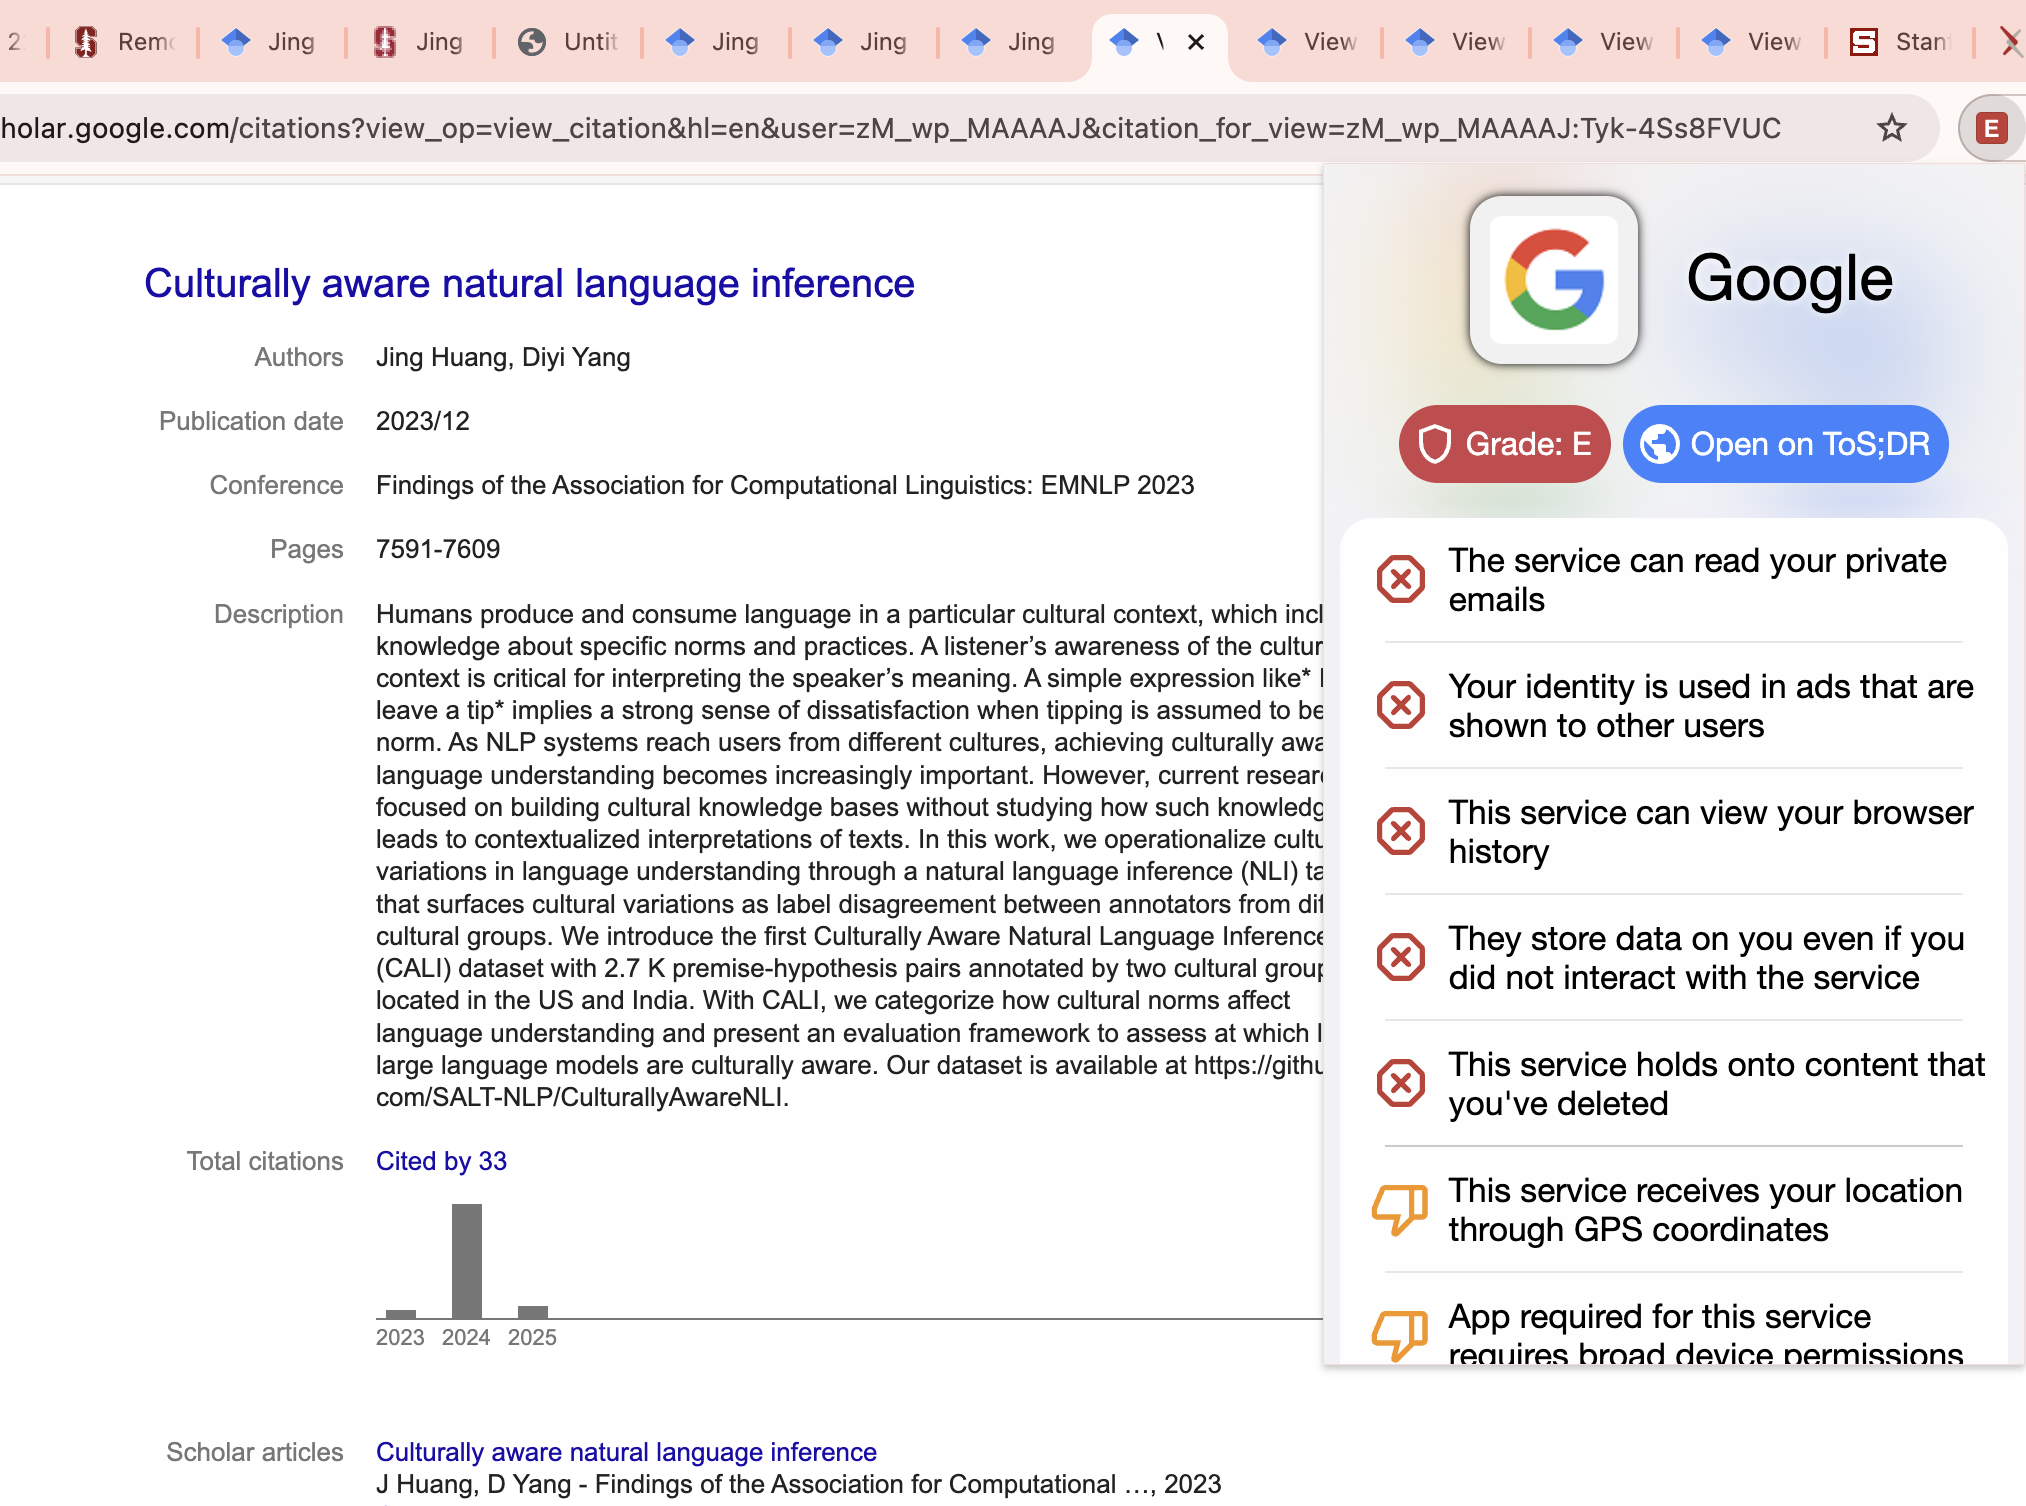
\includegraphics[width=0.75\linewidth]{browser_extension.png}
    \caption{Community Annotated T\&C rating and summaries}
    \label{fig:enter-label}
\end{figure}


\paragraph{Data.}
We will use a community-annotated dataset of T\&C of 500 companies, which qualified attorney vonlunteers have analyzed and labeled. This dataset was previously used to develop a browser extension that show T\&C fairness rating. It also includes Clause-level annotations.

To prepare the dataset for fine-tuning transformer models, we will:\\
	1.	Tokenization \& Cleaning: Standardize legal text we acquired from the company. Remove the date/version mismatches.\\
	2.	Sentence Segmentation: Break long legal clauses into manageable units for NLP models.\\
	3.	Label Normalization: Align fairness ratings with a numerical scale for supervised learning.\\
	4.	Augmentation (if needed): Expand the dataset using semi-supervised techniques like zero-shot prompting from GPT models to generate additional annotations.\\

\paragraph{Methods.}

Our approach involves fine-tuning transformer-based models for legal text summarization and fairness evaluation.\\ 

We will explore and fine-tune pre-trained sequence-to-sequence models to evaluate the best outcome.
We will use Hugging Face transformers to download models.\\
We will train on our annotated dataset, optimizing for text summarization quality and fairness classification accuracy. \\ 
We will implement our legal text pre-processing pipeline, including clause segmentation, tokenization, and explainability analysis. \\
We will compare our model against existing summarization models (e.g., GPT-4, Claude) to assess performance gains.

\paragraph{Baselines.}
We will compare our T\&C summarization model with Pre-trained Transformer Models such as OpenAI ChatGPT 4o, Claude, etc.
We will compare our classifier with the pre-trained classifiers such as LegalBERT and the human expert annotations.

\paragraph{Evaluation.}

We will explore and use various evaluation methods, such as n-gram-based semantic similarity. For the classifier, we plan to use ROC-AUC approaches. 

\paragraph{Ethical Challenges}
Our project presents ethical challenges related to algorithmic bias in legal fairness assessments and misinterpreting AI-generated summaries. We will perform bias audits by cross-checking AI ratings with the community and asking for feedback. We will also put a legal disclaimer that AI summaries are informational, not legal advice, and recommend consulting a lawyer for critical decisions.

\bibliographystyle{unsrt}
\bibliography{references}

\end{document}
